\documentclass[xcolor=dvipsnames, aspectratio=1610]{beamer}
\usetheme{Metropolis}
\usepackage{hyperref}
\usepackage{pgfpages}
\setbeamertemplate{bibliography item}{\insertbiblabel}
\setbeameroption{show notes}
\setbeameroption{show notes on second screen=right}

\title{The Future of Healthcare in a Digitized World}
\author{Noah Wahl}

\begin{document}

\frame{\titlepage}

\begin{frame}{Table of Contents}
    \tableofcontents
\end{frame}

\section{Motivation}%
\label{sec:motivation}

\begin{frame}{\secname}
    \begin{itemize}[<+->]
        \item Healthcare environments slowly adapted to digitization \cite{industryDigitalization}
        \item Chronic and age-related diseases weight heavy on public healthcare \cite{sambamoorthi2015multiple}
        \item Mobile Healthcare has become a large market
        \item AI and ML are emerging in healthcare environments
        \item Value-based healthcare looks very promising
    \end{itemize}
\end{frame}

\section{The Current State of (Digital) Healthcare}%
\label{sec:the_current_state_of_digital_healthcare}

\begin{frame}{\secname}
    \centering
    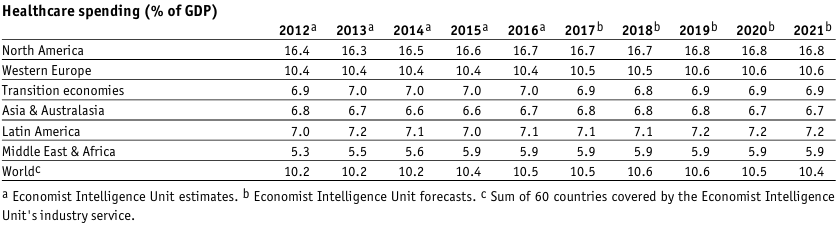
\includegraphics[width=\textwidth]{../media/Screenshot_2020-01-09_01_FULL_REPORT-World_healthcare_and.png} \\
    \small{Healthcare spending around the world \cite{EIU2016}}
\end{frame}
\note[itemize]{
    \item \$7 trillion in 2015, \$8.7 trillion in 2020
    \item 700 deaths and \$21 billion from adverse drug events in the US
}


\begin{frame}{\secname}
    \centering
    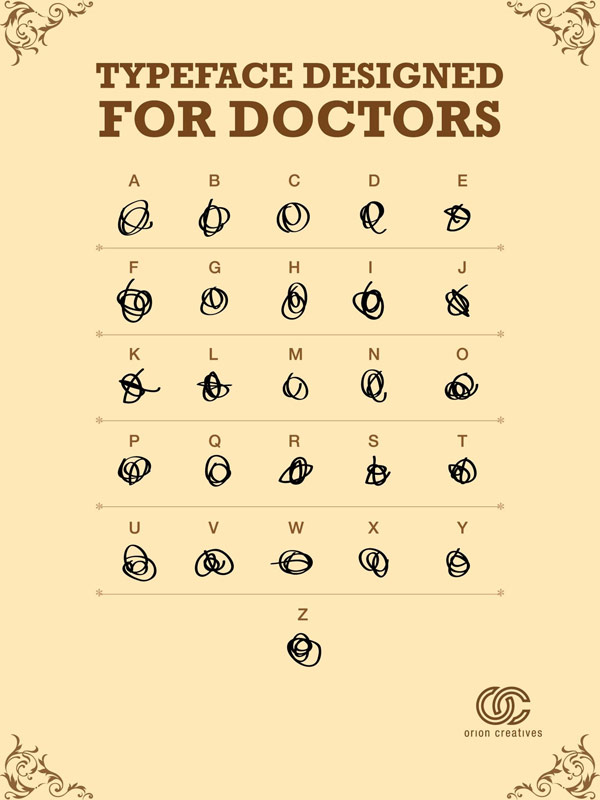
\includegraphics[height=0.8\textheight]{../media/doctor_handwriting.jpg} \\
    \small{This is overplaying the reality, but... \cite{docHandwriting}}
\end{frame}

\note[itemize]{
\item 1 out of 6 words illegible
\item misdiagnosis 225.000 deaths each year in US
}

\section{Smartphones as Digital Healthcare Devices}%
\label{sec:smartphones_as_digital_healthcare_devices}

\begin{frame}{\secname}
    \begin{itemize}[<+->]
        \item Always with us
        \item Many people have activity trackers
        \item Immediate feedback through companion apps
        \item Sensors go as far as monitoring blood sugar levels \cite{glucoseTracker}
        \item Mental health services are rarely well implemented \cite{torous2017needed}
    \end{itemize}
\end{frame}

\note{apps offer real-time capture of environmental context, others try intervention strategies}

\section{Smartphones as Digital Health Inhibitors}%
\label{sec:smartphones_as_digital_health_inhibitors}

\begin{frame}{\secname}
    \begin{itemize}[<+->]
        \item Smartphones use up our cognitive resources \cite{ward2017brain}
        \item Underlying biological cause (oversaturation of dopamine receptors \cite{nieoullon2002dopamine, dopamineRole} and pro-social society \cite{sapiens})
        \item Children and young adults are at a high risk of lasting damage through wrong use of technology \cite{crone2018media}
    \end{itemize}
\end{frame}

\note{prefrontal cortex only fully developed at age 25}

\section{The Future of Digital Healthcare}%
\label{sec:the_future_of_digital_healthcare}

\subsection{Secure Management of Patient Data}%
\label{sub:secure_management_of_patient_data}

\begin{frame}{\secname\ | \subsecname}
    \begin{itemize}[<+->]
        \item Huge amounts of patient data \cite{gopal2019digital}
        \item Stored in data centers with varying levels of security \cite{patil2014big}
        \item Need common data representations, local and regional standards \cite{patil2014big}
        \item This allows secure protocols for transportation and analysis in real-time \cite{patil2014big}
        \item For IoT environments with their tight resource-constraints this requires further messurements, e.g. scaling key management solutions \cite{patil2014big}
        \item Data should be anonymized prior to analytics
    \end{itemize}
\end{frame}

\note[itemize]{
\item many manufacturers of IoT devices send them out with default settings that are not changed by the buyers
\item imagine WannaCry-like attack with IoT devices
\item WannaCry hit the UKs NHS hospitals with 70.000 devices including computers, MRI scanners and blood-storage refrigerators
\item PKI has to be automated to manage certificates on this scale
}

\subsection{Individually Tailored Care}%
\label{sub:individually_tailored_care}

\begin{frame}{\secname\ | \subsecname}
    \begin{itemize}[<+->]
        \item More and more AI-based algorithms are accepted by healthcare administrations \cite{fdaAi}
        \item Use is limited due to lack of suitable data, e.g. image processing software for cancer detection \cite{kiKroenung}
        \item Google, Apple and Co. have the algorithms as well as the data
        \item Their devices have all the information they need from body sensors and in future, implants, to find immediate solutions or get feedback from similar cases from a data center \cite{kiKroenung}
        \item Implants include blood glucose monitoring devices that release insulin into the bloodstream accordingly \cite{rege2017development}
        \item AI-based medical services outside of traditional healthcare environments are likely to be the future
    \end{itemize}
\end{frame}

\note[itemize]{
\item most are in radiology and cardiology
\item AI-based medical services will be patient driven and provided by big companies on the private market
}

\subsection{Value-Based Healthcare}%
\label{sub:value_based_healthcare}

\begin{frame}{\secname\ | \subsecname}
    \begin{itemize}[<+->]
        \item Our leading killers are almost exclusively incommutable diseases which account for around 75\% of global health expenditure \cite{tsiachristas2016financial}
        \item These diseases do not kill their victims until several years after diagnosis
        \item Living with these diseases has not only an effect of peoples physical well-being, but also their mental health
        \item Value-based healthcare seeks to prevent these diseases and even if they occur, create value from healthcare outcomes relative to the costs of the treatment \cite{putera2017redefining}
        \item Digitization comes to play here as a tool to educate medical professionals as well as individuals about preventive measurements to achieve better health outcomes
        \item To give recommendations weight, AI is used in studies and clinical trials to detect correlation and causation that human analytics may oversee \cite{rehme2014identifying}
    \end{itemize}
\end{frame}

\note{Studies that use ML methods to assist stroke diagnosis reach accuracy of almost 90\%}

\section{Conclusion}%
\label{sec:conclusion}

\begin{frame}{\secname}
    \begin{itemize}[<+->]
        \item Healthcare is expensive, inefficient and ineffective as of now
        \item Mobile healthcare promisses a partial solution
        \item AI and ML are coming, but they will not magically solve the problem
        \item A common data representation is needed to effectively use these algorithms
        \item Value-based healthcare can use digitization to revolutionize healthcare
    \end{itemize}
\end{frame}

%references

\begin{frame}[allowframebreaks]{References}
    \bibliographystyle{abbrv}
    \bibliography{references}
\end{frame}
\end{document}
